\chapter{Micro Tasks}\label{Chapter:datasets}
In the chapter \ref{Chapter:proposals} we saw that AG exhibits compositional learning and can learn PCFG rules when explicitly asked to do so. We can now test if it can infer the rules of the grammar behind a formal language from the dataset and then generalize to unseen strings generated using the grammar in a zero-shot fashion. Since it has already been seen in chapter \ref{Chpater:intro} that \cite{Lake2017} introduced the SCAN domain which is essentially a context free language showed that vanilla seq2seq models can't learn the rules governing this dataset in a systematic fashion. It stands to reason that instead of directly testing the compositional abilities of my method on a context free language which is still higher up in the Chomsky Hierarchy, I start with the much simpler domain of sub-regular languages.

CommAI mini tasks \citep{Baroni2017} are a set of strictly local and locally testable (please refer to section \ref{flt:sh}) languages designed to test the generalization capabilities of a compositional learner. Based on the mini tasks we propose a new dataset of sub-regular languages which we call the Micro Tasks. While the CommAI mini task position themselves as strictly local and locally testable tasks of progressive difficulty we add another layer of difficulty to the tasks by setting them up as either a decision problem (verify) or search problem (produce) in the same training domain.

\textbf{Search vs Decision} - It has been shown that for a general language $L \in NP$ search is more difficult than decision \cite{Bellare1994}. The \textit{verification} task is clearly a decision problem while the \textit{production} task is a search problem. Since Micro tasks fall into the domain of sub-regular languages they can be decided at-most in the linear time of length of string by a finite state automaton (section \ref{flt:ch}), they clearly are $\notin NP$. However it still makes sense to analyze whether for a prover (seq2seq network, lstm etc.) is the task of computing the witness for the membership in a $L \notin NP$ more difficult than establishing the existence of such a witness.

The \textbf{verify} task input is of the form \lq $\langle$ string of k-factors $\rangle$ verify $\langle$ witness $\rangle${}\rq\ with the output being a standard classification token \lq yes/no{}\rq\. The witness string is of length $\geq$ the given k-factor string, and a model must verify if the k-factors exist in the witness. The \textbf{production} task consists of an input of the form \lq $\langle$ string of k-factors $\rangle$ produce\rq{} with the output being a satisfying assignment (equal to the length of the given string) to the criteria laid out in the input string.

Any given $\langle$ k-factor string $\rangle$ in either of the verify or produce tasks can be one out of the following four types:
\begin{itemize}
	\item \textbf{atomic}\footnote{This is present only in the verify task since in produce it just becomes a unary k-factor without any operator and produces an output which is a copy of itself. It is like the \lq and\rq{} task without any operator or additional symbols in the input.} - consists of a single word/k-factor/n-gram from the vocabulary and task of a learner is either to check the existence of this k-factor in the witness (verify task) or produce exactly this k-factor as target (production) task. In the verification setting this task is strictly local in its description (section \ref{flt:sh}) and can be solved by scanner with an access to the witness/lookup-table.
	\item \textbf{or} - consists of k-factors joined by the boolean operator \lq or \rq{}. This task is again strictly local in its description albeit more memory intensive than the atomic task because it requires storage of multiple k-factors in memory.
	\item \textbf{and} - consists of k-factors joined by the boolean operator \lq and \rq{}. Now a learner doesn't simply have to verify the existence of a single k-factor in the witness. Instead for each k-factor it has to maintain a record of it's occurence/non-occurence in the witness, and thus requires store of all k-factors in memory. This task is therefore locally k-testable. 
	\item \textbf{not} - consists of k-factors acted upon by both \lq and \rq{} as well as \lq not \rq{} operators. While the \textit{conjunction} acts upon two k-factors, the \textit{negation} only acts upon one. This task also has a locally k-testable description. 
\end{itemize}



\section{Data  Structure}
Out of the 128 ascii characters, only 100 are printable and of those 100, 6 refer to newline, space, tab etc. which are not directly observable and therefore our vocabulary $\Sigma$ consists of 94 printable ascii characters and two binary output tokens \lq yes\rq{} and \lq no\rq{}. The vocabulary is split into two equal disjoint subsets. The train and various test sets constructed from this vocabulary are as follows:
\begin{enumerate}
	\item \textbf{train} consists of 120000 pairs of input output symbols with input composition length (vocabulary symbols excluding operators) ranging between $\langle$ 2 and 4 $\rangle$ (limits inclusive). $10\%$ of this data is used to create the validation set. Any particular input composition is constructed using words from only one of the subsets.
	\item \textbf{unseen test} consists of 12000 i/o pairs with input composition length ranging between $\langle$ 2 and 4 $\rangle$. The compositions are created by randomly sampling words from both subsets of the vocabulary i.e cross-composition between subsets is allowed
	\item \textbf{longer test} consists of i/o pairs such that input composition length is between $\langle$ 5 and 7 $\rangle$ (limits inclusive). cross-composition of words from two different subsets isn't allowed.
	\item \textbf{unseen longer test} consist of i/o pairs such that input composition length is between $\langle$ 5 and 7 $\rangle$ and cross-composition is allowed.
\end{enumerate}

The distribution of the boolean operators (i.e. the number of tasks per operator) in the train and unseen test set (the distribution is same for every test set) can be seen in figures \ref{micro_train} and \ref{micro_test} respectively.

\begin{figure}[ht] 
	\begin{subfigure}[b]{0.5\linewidth}
		\centering
		\ifpdf
		\includegraphics[width=0.95\linewidth]{./figs/micro/train_verify-pdf}
		\else
		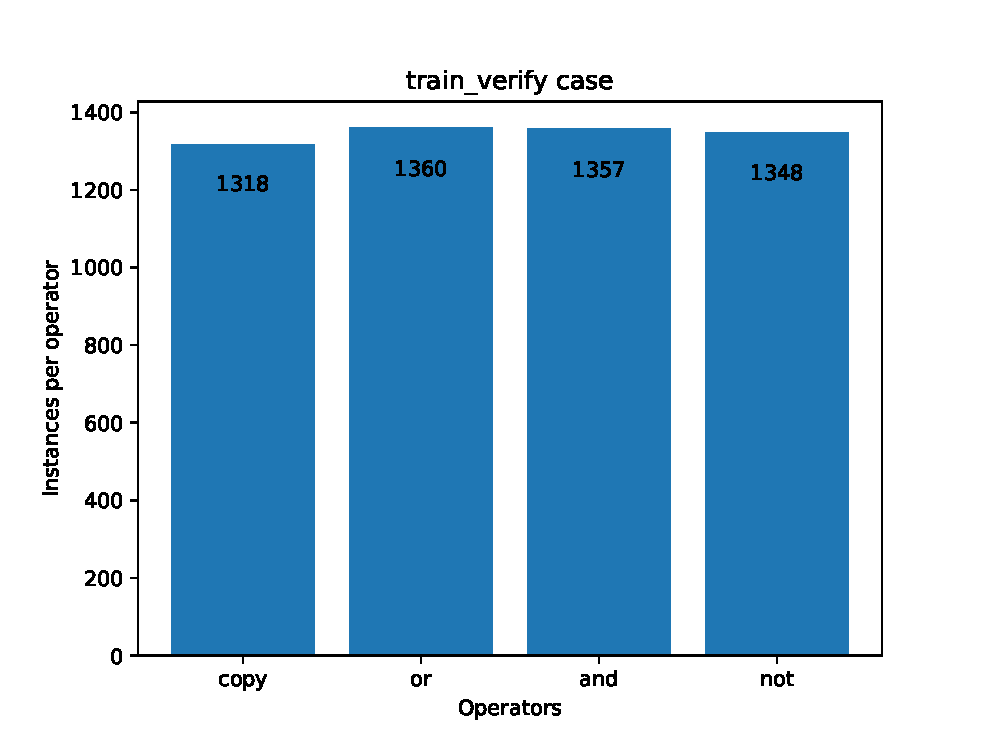
\includegraphics[width=0.95\linewidth]{./figs/micro/train_verify-eps}
		\fi
		\caption{Verification Task} 
		\label{tr_ver} 
		\vspace{2ex}
	\end{subfigure}%% 
	\begin{subfigure}[b]{0.5\linewidth}
		\centering
		\ifpdf
		\includegraphics[width=0.95\linewidth]{./figs/micro/train_produce-pdf}
		\else
		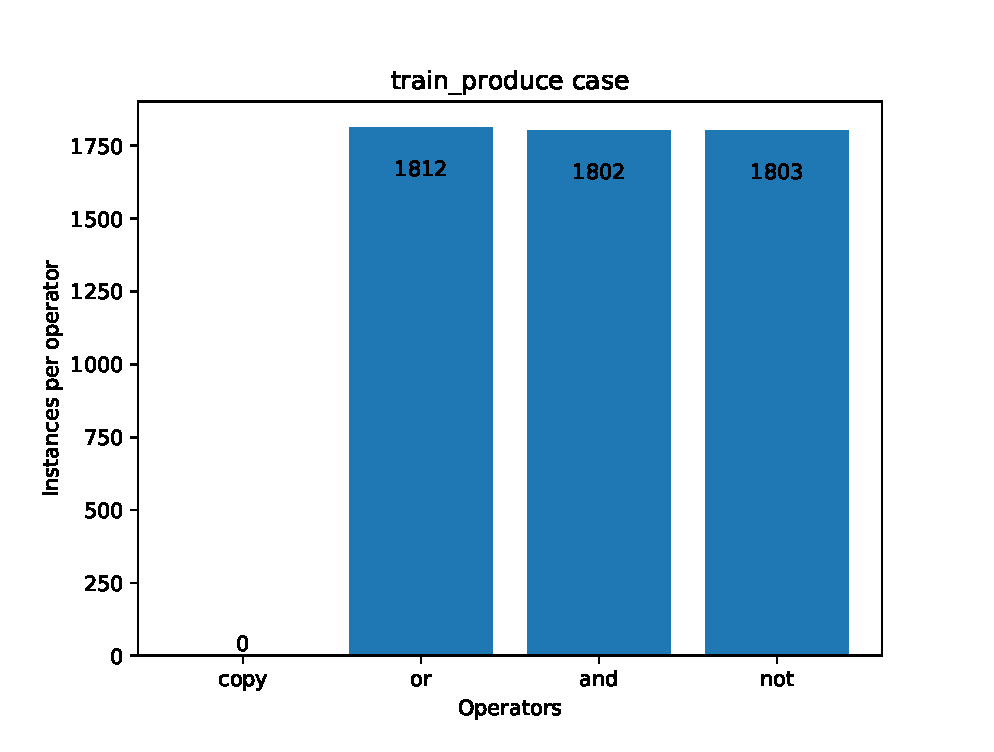
\includegraphics[width=0.95\linewidth]{./figs/micro/train_produce-eps}
		\fi 
		\caption{Production Task} 
		\label{tr_prd} 
		\vspace{2ex}
	\end{subfigure}
	\caption{Micro Tasks - Training Data}
	\label{micro_train}
\end{figure}

\begin{figure}[ht] 
	\begin{subfigure}[b]{0.5\linewidth}
		\centering
		\ifpdf
		\includegraphics[width=0.95\linewidth]{./figs/micro/unseen_verify-pdf}
		\else
		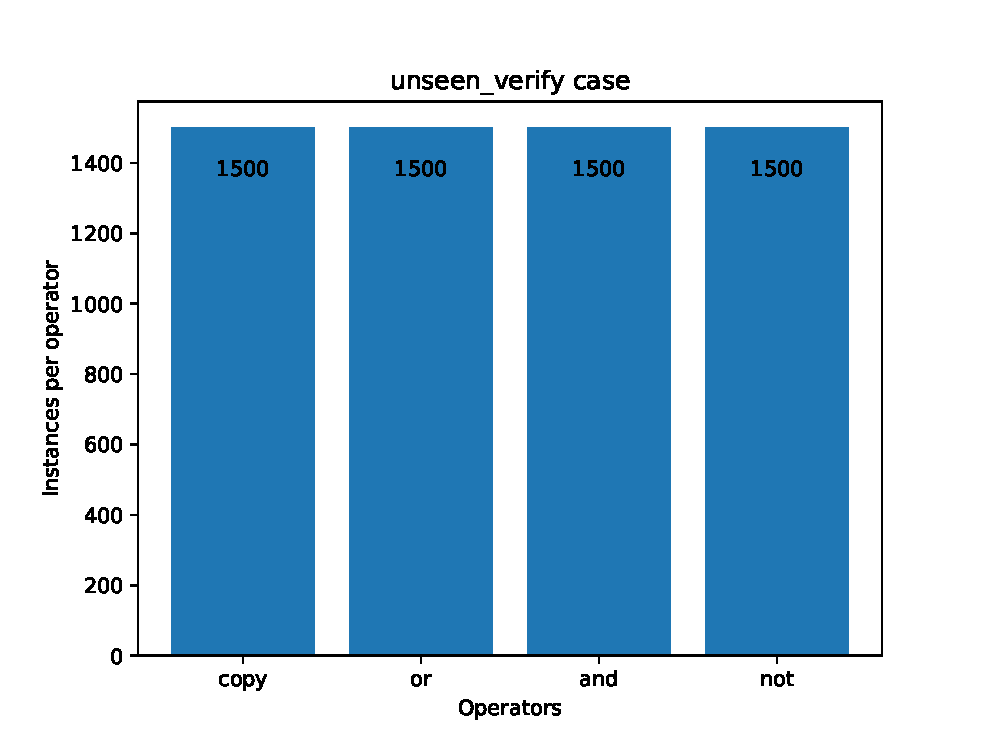
\includegraphics[width=0.95\linewidth]{./figs/micro/unseen_verify-eps}
		\fi
		\caption{Verification Task} 
		\label{un_ver} 
		\vspace{2ex}
	\end{subfigure}%% 
	\begin{subfigure}[b]{0.5\linewidth}
		\centering
		\ifpdf
		\includegraphics[width=0.95\linewidth]{./figs/micro/unseen_produce-pdf}
		\else
		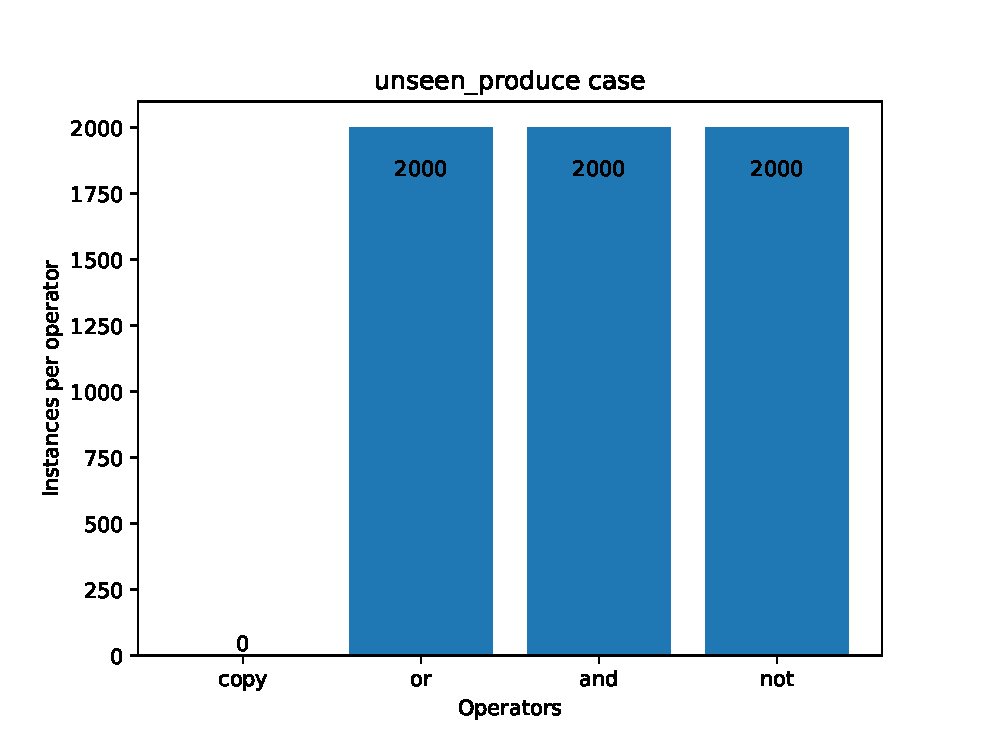
\includegraphics[width=0.95\linewidth]{./figs/micro/unseen_produce-eps}
		\fi 
		\caption{Production Task} 
		\label{un_prd} 
		\vspace{2ex}
	\end{subfigure}
	\caption{Micro Tasks - Unseen Data}
	\label{micro_test}
\end{figure}

% Examples of verify and produce tasks in each of the data-split is presented in tables \ref{mt:stats:ver} and \ref{mt:stats:prod}.
%\begin{table}[ht]
%	\centering
%	\begin{tabular}{l|lc}
%		& Example & Size\\
%		\hline
%		train & \ and K verify y  & 54000 \\
%		unseen test & b or X or D or a verify < D f & 6000 \\
%		longer test & E or H or E or ] or ! verify & E d ] !  & 6000 \\
%		unseen longer test & ^ and U and T and . and X and D and S verify D S s ^ # T . U X & 6000 \\
%	\end{tabular}
%	\caption{Micro Tasks Verify Splits}
%	\label{mt:stats:ver}
%\end{table}
%
%\begin{table}[ht]
%	\centering
%	\begin{tabular}{l|lc}
%		& Example & Size\\
%		\hline
%		train & r and not G and W produce  & 54000 \\
%		unseen test & N and X produce & 6000 \\
%		longer test & y or n or t or y or [ produce & 6000 \\
%		unseen longer test & ] and z and } and I and 5 and not f produce & 6000 \\
%	\end{tabular}
%	\caption{Micro Tasks Produce Splits}
%	\label{mt:stats:prod}
%\end{table}


\section{Experimental Setup}

\subsection{AG Trace}
The trace for the hard guidance of micro-tasks is different for verify and produce cases owing to the fact that verify has a single emission (yes/no token) while produce has multiple emissions. Furthermore pondering is explicitly mocked here by augmenting the output with a ponder token. The ponder token helps the network in focusing on the summarization of the entire string and the meta-information i.e. verify/produce, before moving on to the emission of the actual targets. The details of the trace are as follows:

\textbf{Verify}. Here we have a trace of length 3 with the focus at end of string, meta-information and end of witness respectively. While the first two indices of the trace correspond to the ponder tokens in the output, the last index corresponds to the decision token which is the actual target. The trace is visualized in figure \ref{ag_ver}.

\textbf{Produce}.In the case of produce while the ponder tokens and the trace corresponding to them remain the same as in the case of verify the trace corresponding to the emissions changes. The trace corresponds to the index in input string for an emission in output string. In the case of not, every emission in target which isn't in input is traced in ascending order of index of the words in input which are acted upon by a not operator. The trace is visualized in figure \ref{ag_prd}

\begin{figure}[ht] 
	\begin{subfigure}[b]{0.5\linewidth}
		\centering
		\ifpdf
		\includegraphics[width=0.95\linewidth]{./figs/micro/ver-pdf}
		\else
		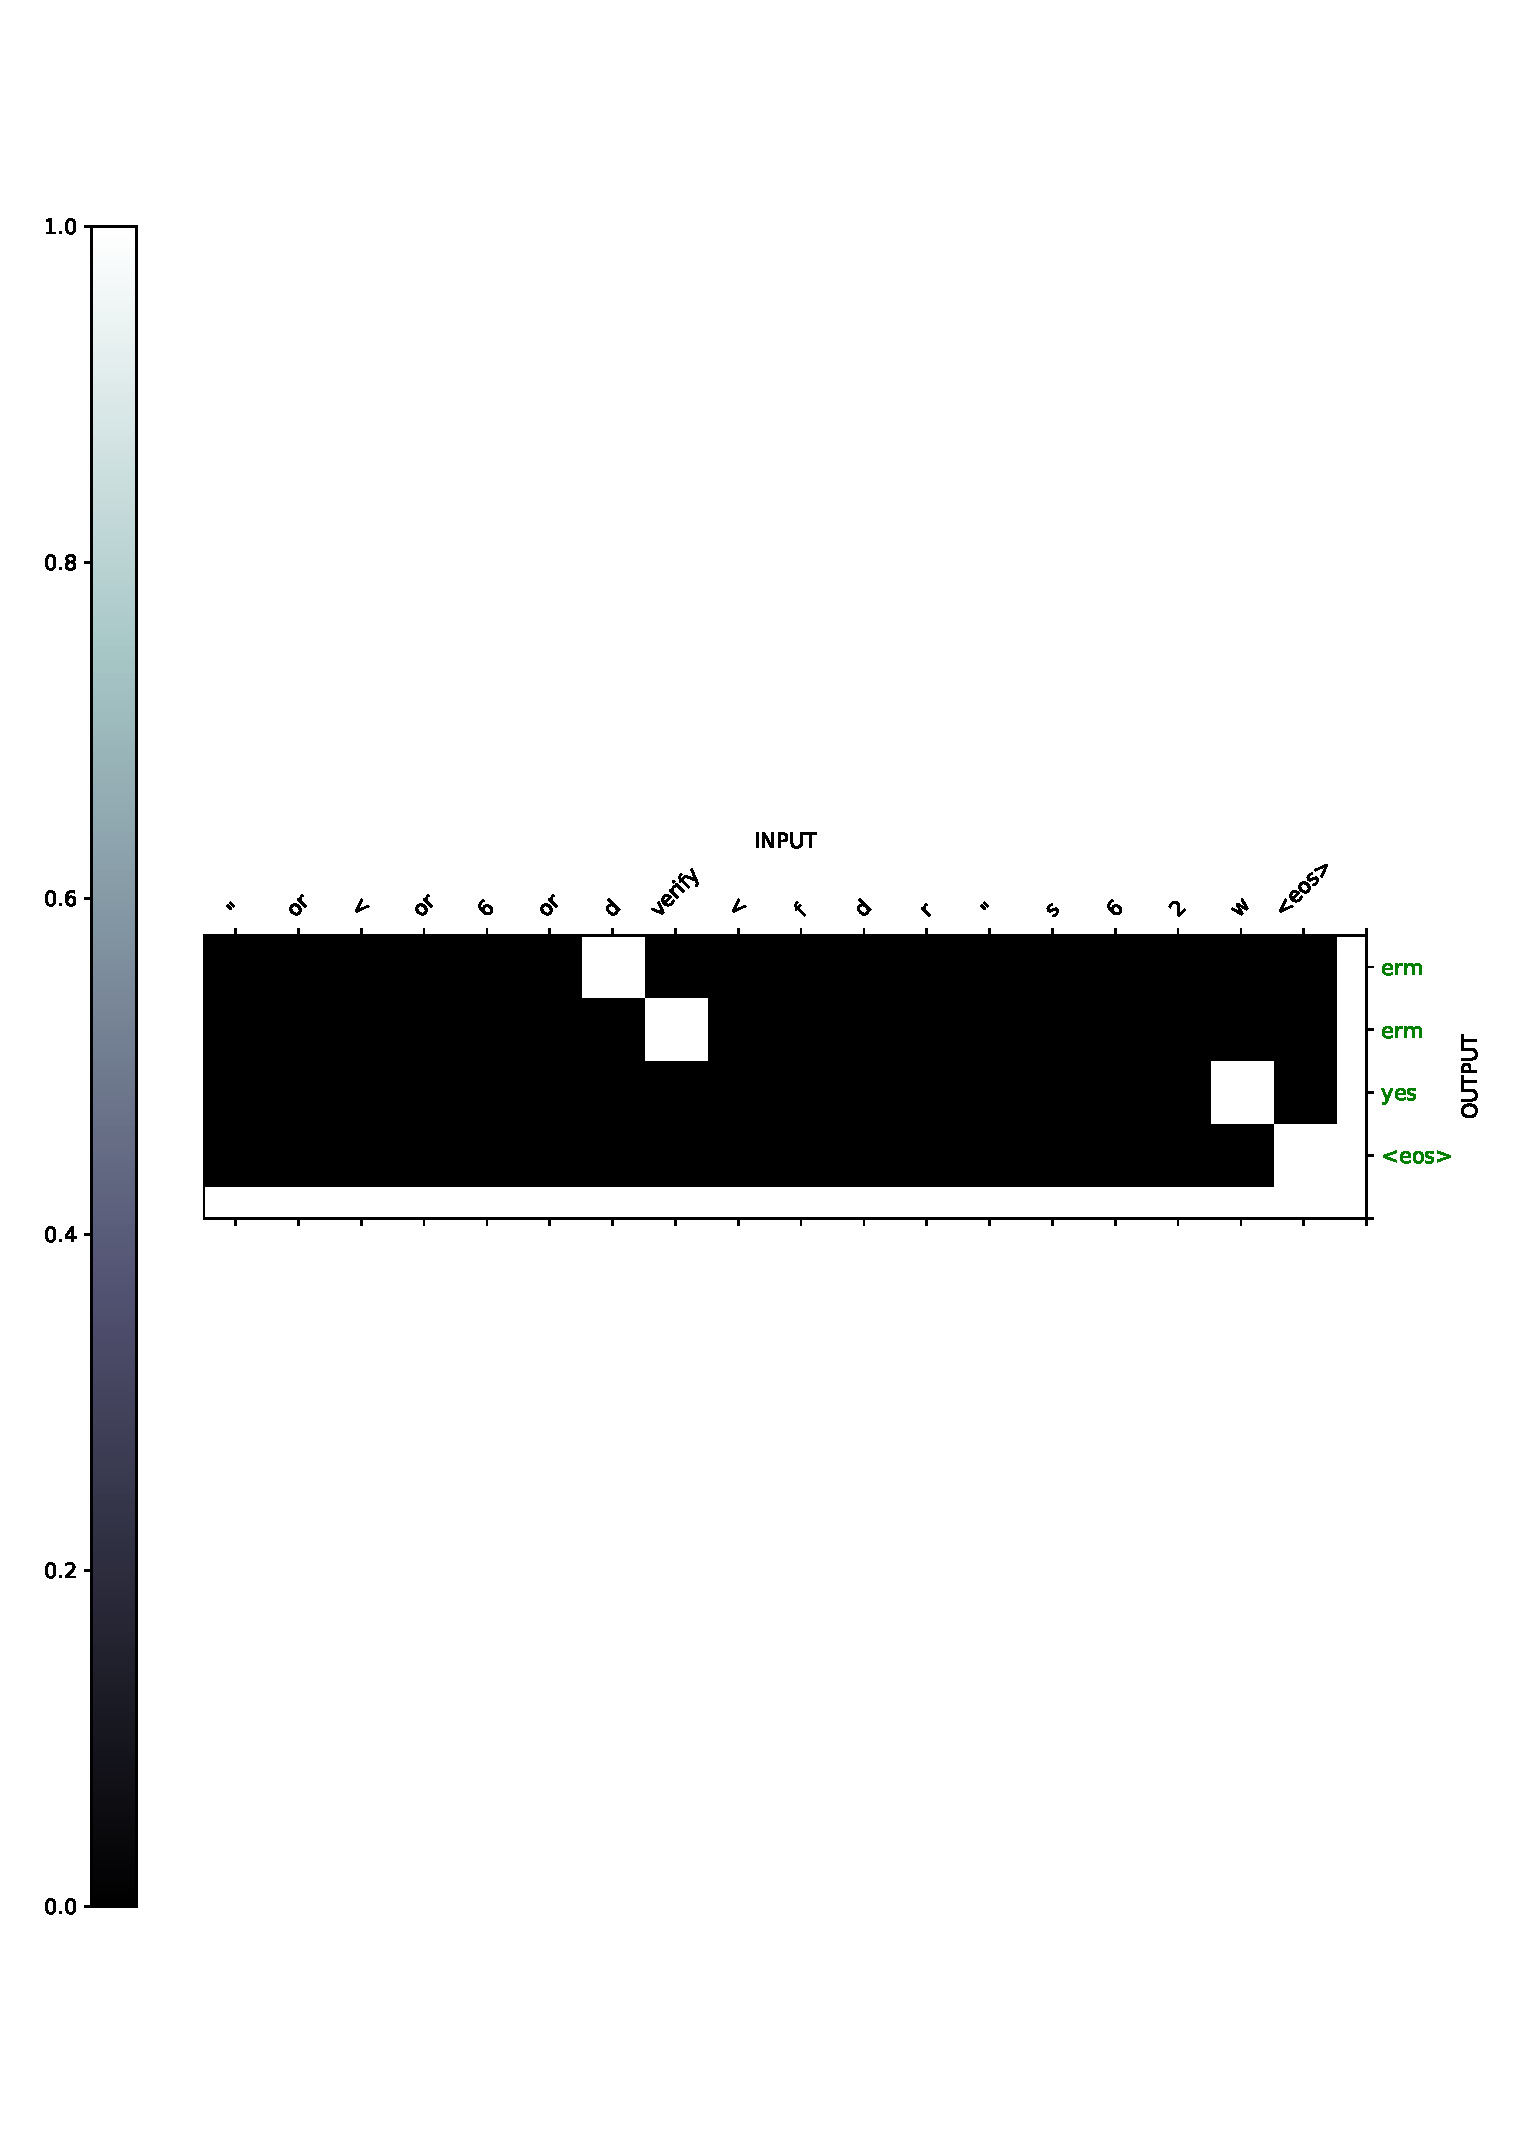
\includegraphics[width=0.95\linewidth]{./figs/micro/ver-eps}
		\fi
		\caption{AG Trace for Verification Task} 
		\label{ag_ver} 
		\vspace{2ex}
	\end{subfigure}%% 
	\begin{subfigure}[b]{0.5\linewidth}
		\centering
		\ifpdf
		\includegraphics[width=0.95\linewidth]{./figs/micro/prof-pdf}
		\else
		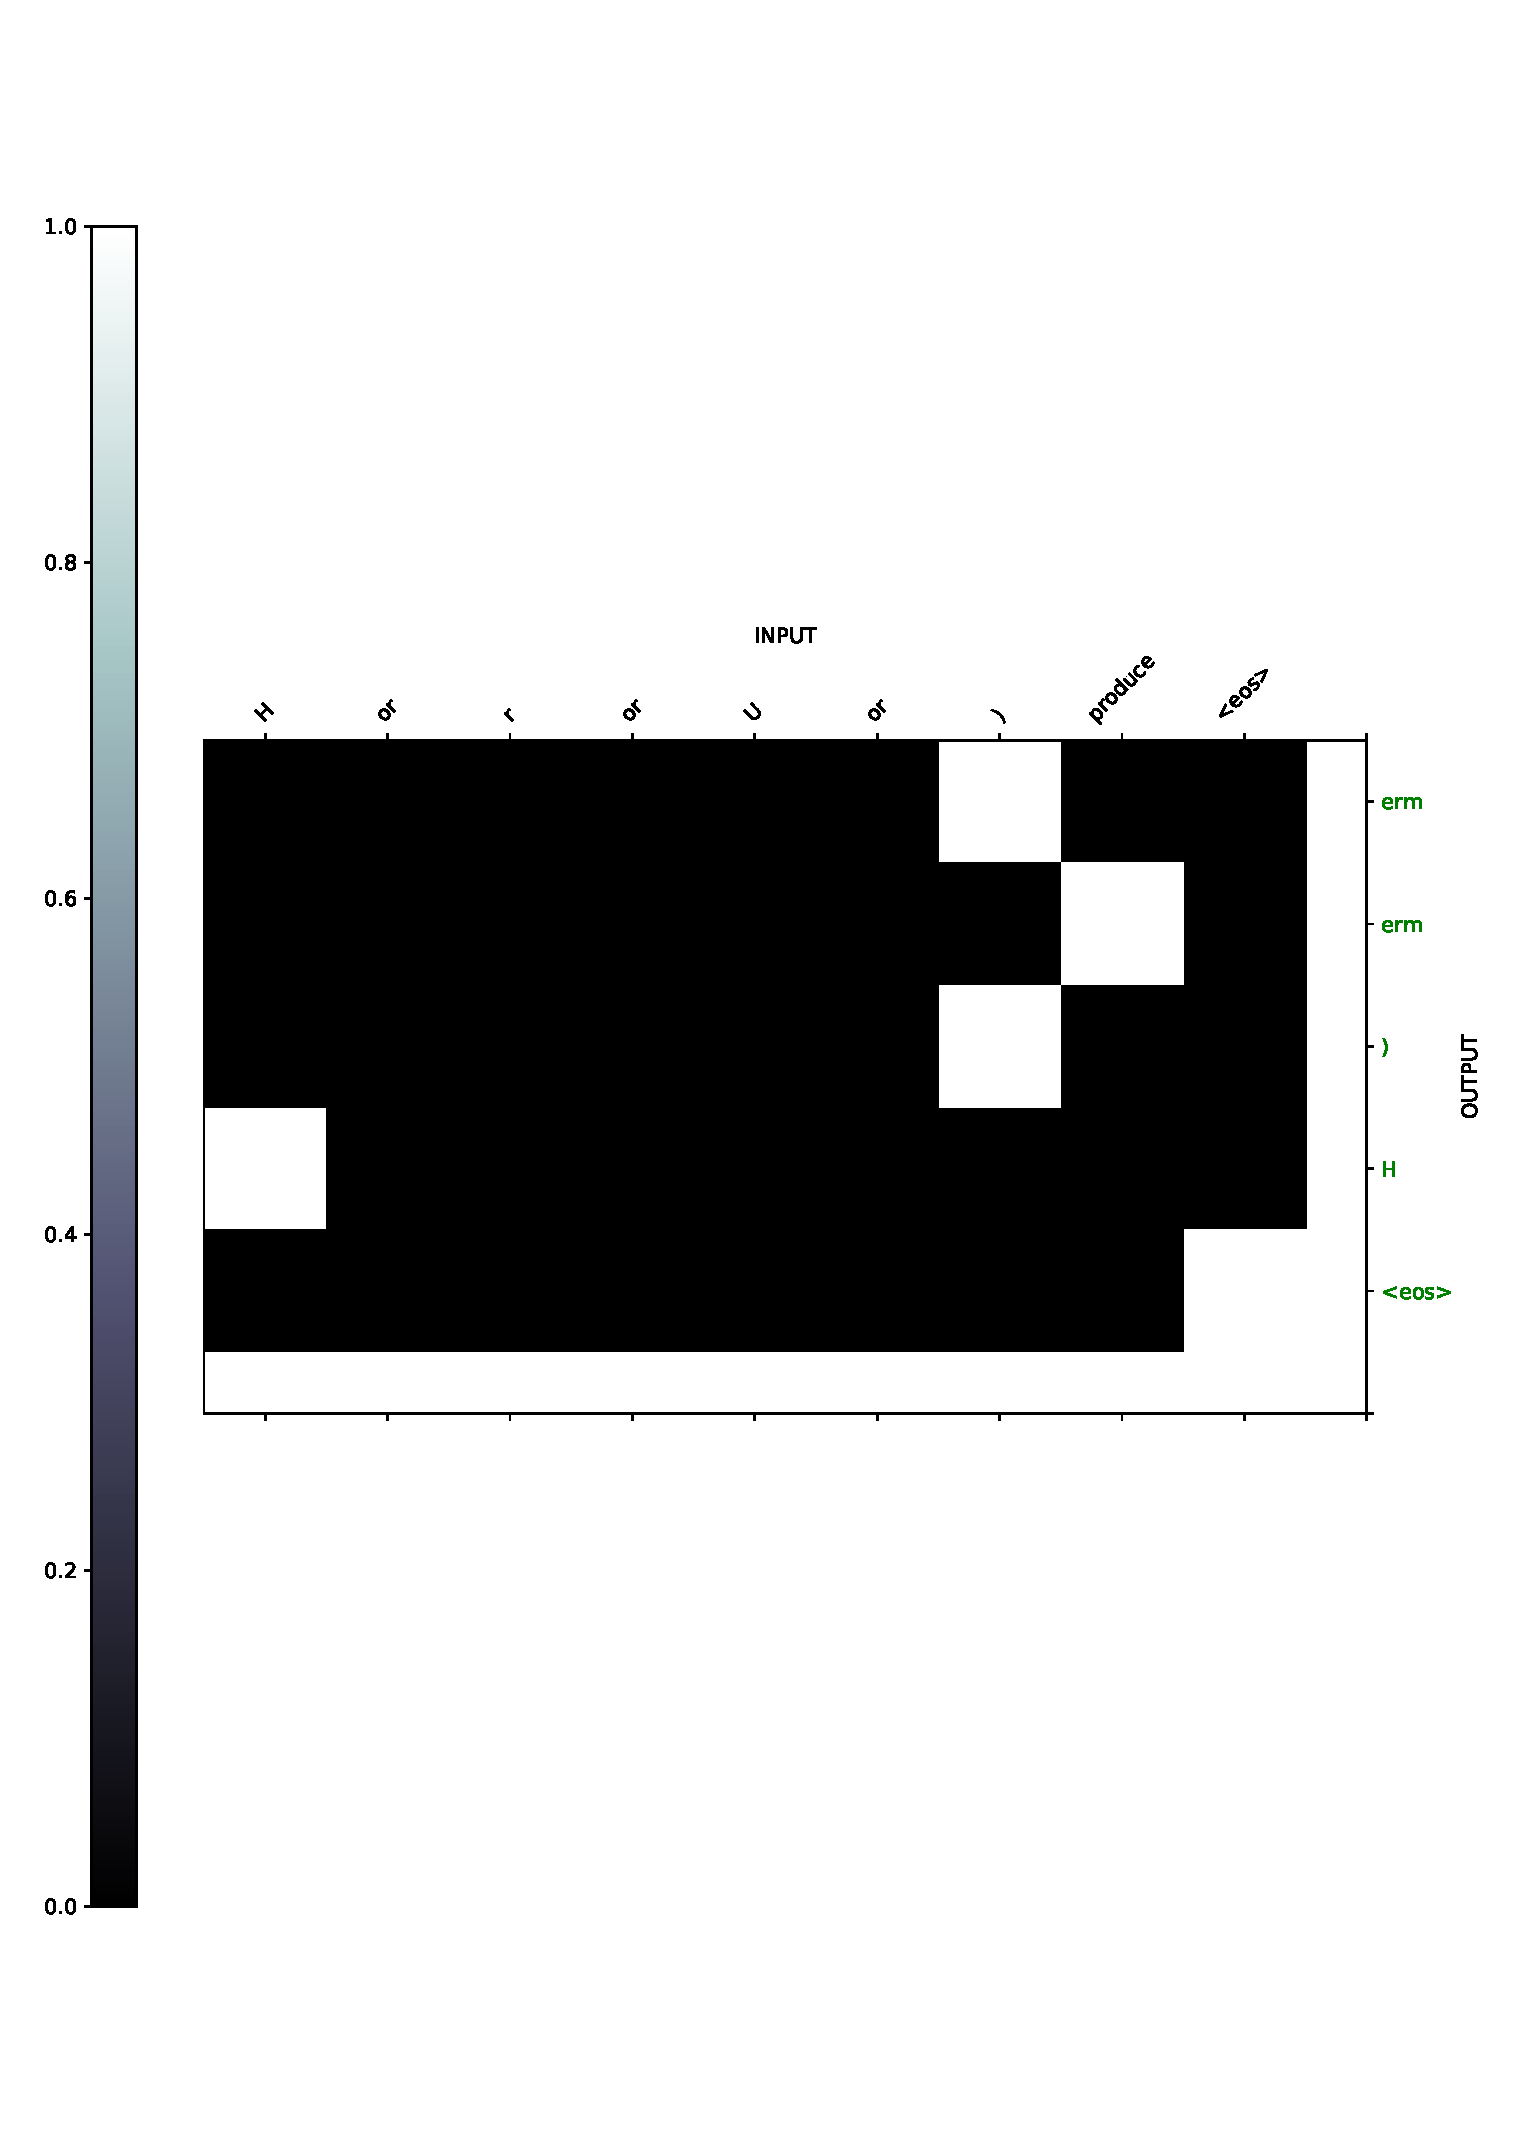
\includegraphics[width=0.95\linewidth]{./figs/micro/prod-eps}
		\fi 
		\caption{AG Trace for Production Task} 
		\label{ag_prd} 
		\vspace{2ex}
	\end{subfigure}
	\caption{Micro Tasks - Attentive Guidance Trace}
	\label{mt_trace}
\end{figure}

\subsection{Micro task Accuracy}
Similar to the symbol rewriting dataset (section \ref{datasets:sr}) micro tasks is a probabilistic dataset in both the number and order of emissions. Therefore just as we had to define a symbol rewriting metric in section \ref{sr:acc_desc} we need to define a new accuracy measure for microtasks. While the microtask accuracy for verify task is simply contingent on the final emission, which is binary, the accuracy for \lq or \rq{}, \lq and \rq{}, \lq not \rq{}, tasks are separately defined as follows:

\begin{itemize}
	\item \textbf{or} - by checking the presence of any of the input token in predicted sequence.
	\item \textbf{and} - by checking the presence of all of the input tokens in predicted sequence.
	\item \textbf{not} - by ensuring that the set of all the input tokens preceded by negation and the predicted sequence are disjoint. This is followed by the same test as above for all the tokens not preceded by negation. 
\end{itemize}

\subparagraph{Hyperparameters} Three different kindof models- baseline(vanila seq2seq), learned guidance(attentive guidance) and hard guidance (attention vectors explicitly provided at decoding) were trained on this dataset using same hyperparameters. The hyperparameters used for the experiments were : rnn cell = lstm, hidden layer size = embedding size = 128, attention =pre-rnn \citep{Bahdanau2014}, alignment measure = mlp, optimizer=Adam \citep{KingmaB14}, learning rate = 0.001.

\section{Micro Tasks - Results}
Since the dataset is probabilistic in nature, it is reasonable to create multiple splits of the data and train different models on each split. I generated 5 different train and test splits of the data and trained separate baselines, learned and hard guided models on each of these splits. Each of these trained models were then used to get the accuracies on the 5 test splits.The mean of these accuracy values along with the error bars (max, min) values is presented for each operation individually in for both verify and produce tasks.

\begin{figure}[ht] 
	\begin{subfigure}[b]{0.5\linewidth}
		\centering
		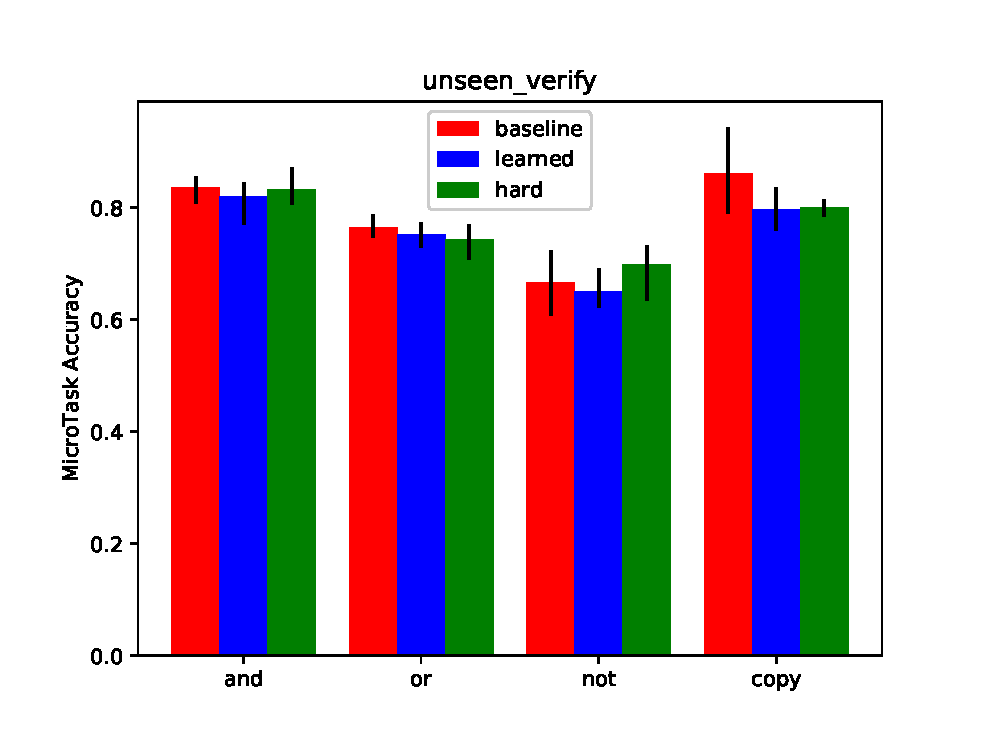
\includegraphics[width=0.95\linewidth]{./figs/micro/unseen_verify}
		\caption{Accuracies for verify task } 
		\label{mtu1} 
		\vspace{2ex}
	\end{subfigure}%% 
	\begin{subfigure}[b]{0.5\linewidth}
		\centering
		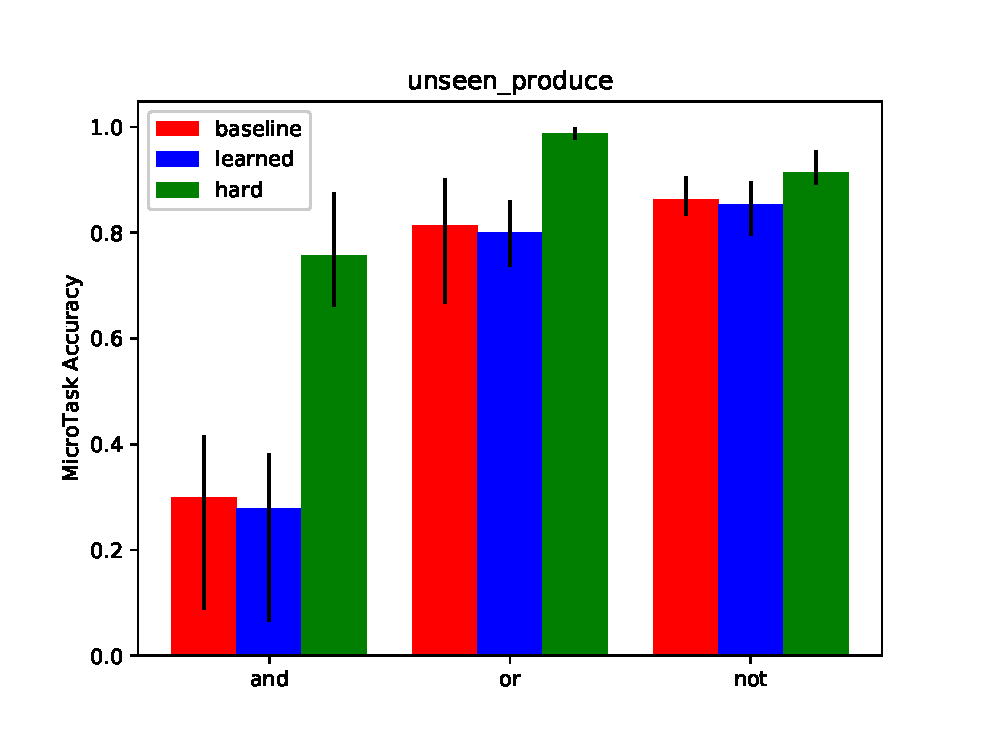
\includegraphics[width=0.95\linewidth]{./figs/micro/unseen_produce}
		\caption{Accuracies for produce task } 
		\label{mtu2} 
		\vspace{2ex}
	\end{subfigure}
	\caption{Micro Task accuracies per operation for unseen test }
	\label{mtu}
\end{figure}
A general observation from these results is that on the verify task all the models have similar optimum values, for each of the operations. The best results are for the \lq and\rq{} \& \lq copy/atomic\rq{} tasks. It can be argued that these two operations exhibit lower stochasticity than the remaining two operations in the sense that the symbols/morphemes that the model is expected to look for remain fixed in the witness string. This isn't the case for the \lq or\rq{} \& \lq not\rq{} tasks and thus for a verifier \lq not\rq{} is arguably the most difficult operation in the verification task. The results on each of the test splits (figures \ref{mtu1},\ref{mtl1} and \ref{mtul1}) expectedly concur with this hypothesis.
\begin{figure}[ht] 
	\begin{subfigure}[b]{0.5\linewidth}
		\centering
		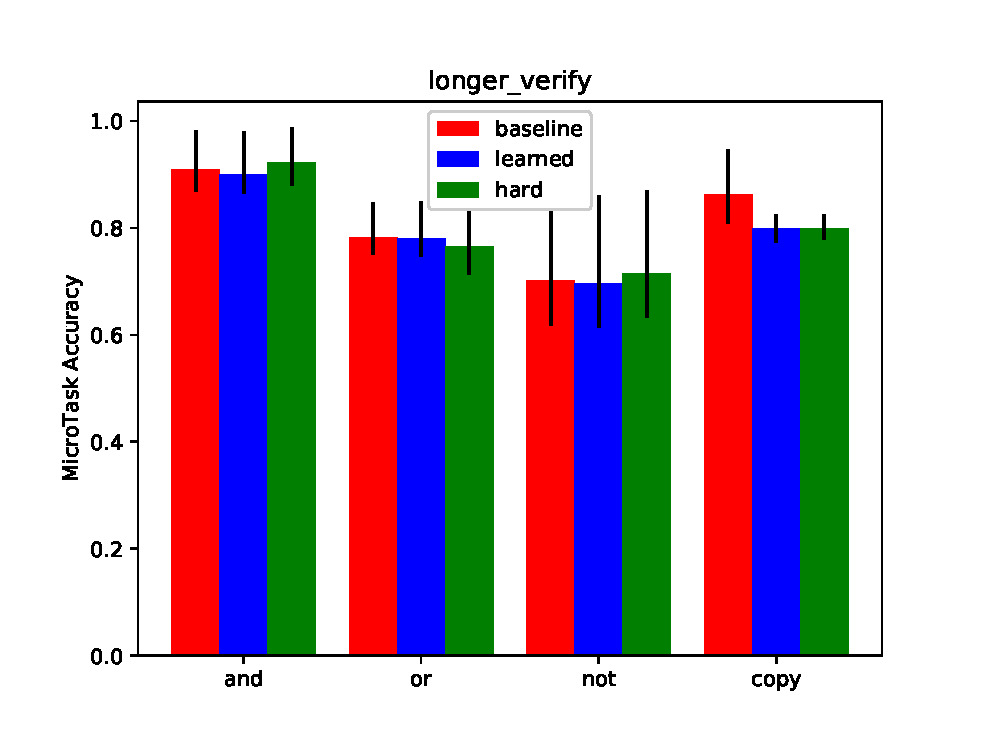
\includegraphics[width=0.95\linewidth]{./figs/micro/longer_verify}
		\caption{Accuracies for verify task } 
		\label{mtl1} 
		\vspace{2ex}
	\end{subfigure}%% 
	\begin{subfigure}[b]{0.5\linewidth}
		\centering
		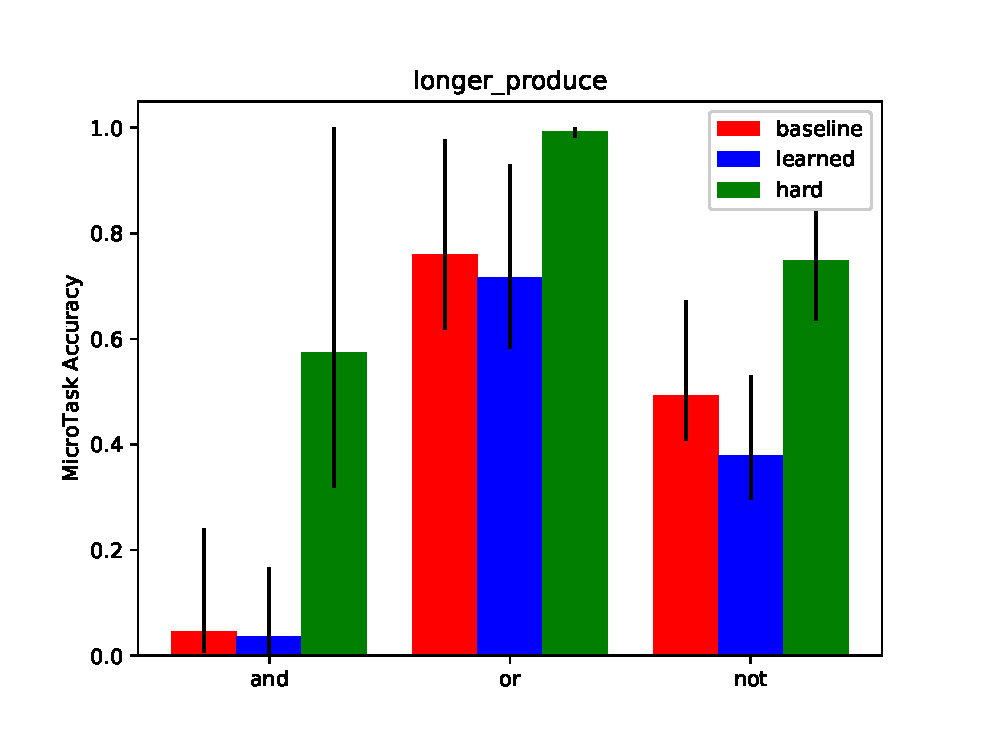
\includegraphics[width=0.95\linewidth]{./figs/micro/longer_produce}
		\caption{Accuracies for produce task } 
		\label{mtl2} 
		\vspace{2ex}
	\end{subfigure}
	\caption{Micro Task accuracies per operation for longer test }
	\label{mtl}
\end{figure}

\begin{figure}[ht] 
	\begin{subfigure}[b]{0.5\linewidth}
		\centering
		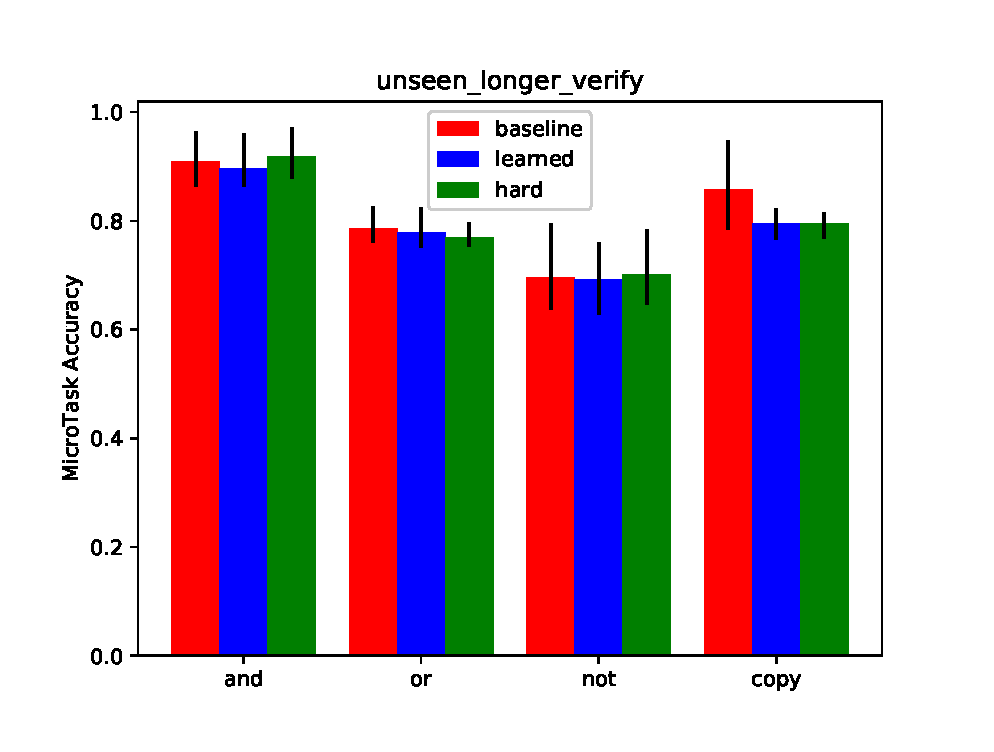
\includegraphics[width=0.95\linewidth]{./figs/micro/unseen_longer_verify}
		\caption{Accuracies for verify task } 
		\label{mtul1} 
		\vspace{2ex}
	\end{subfigure}%% 
	\begin{subfigure}[b]{0.5\linewidth}
		\centering
		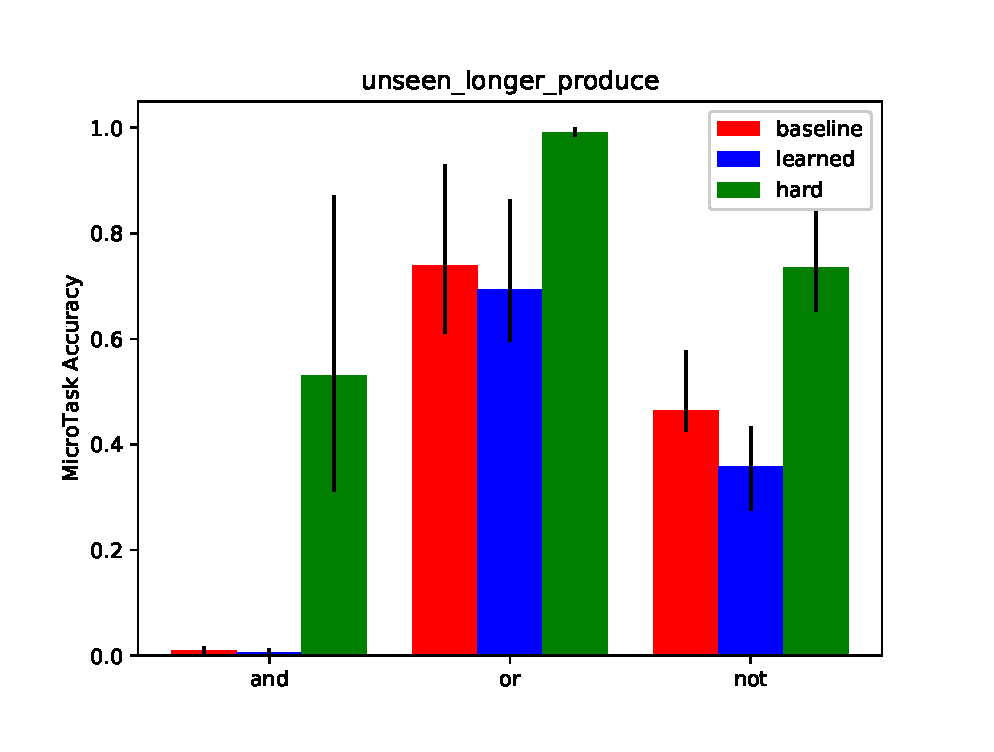
\includegraphics[width=0.95\linewidth]{./figs/micro/unseen_longer_produce}
		\caption{Accuracies for produce task } 
		\label{mtul2} 
		\vspace{2ex}
	\end{subfigure}
	\caption{Micro Task accuracies per operation for unseen longer test }
	\label{mtul}
\end{figure}


\begin{figure}[ht] 
	\begin{subfigure}[b]{0.5\linewidth}
		\centering
		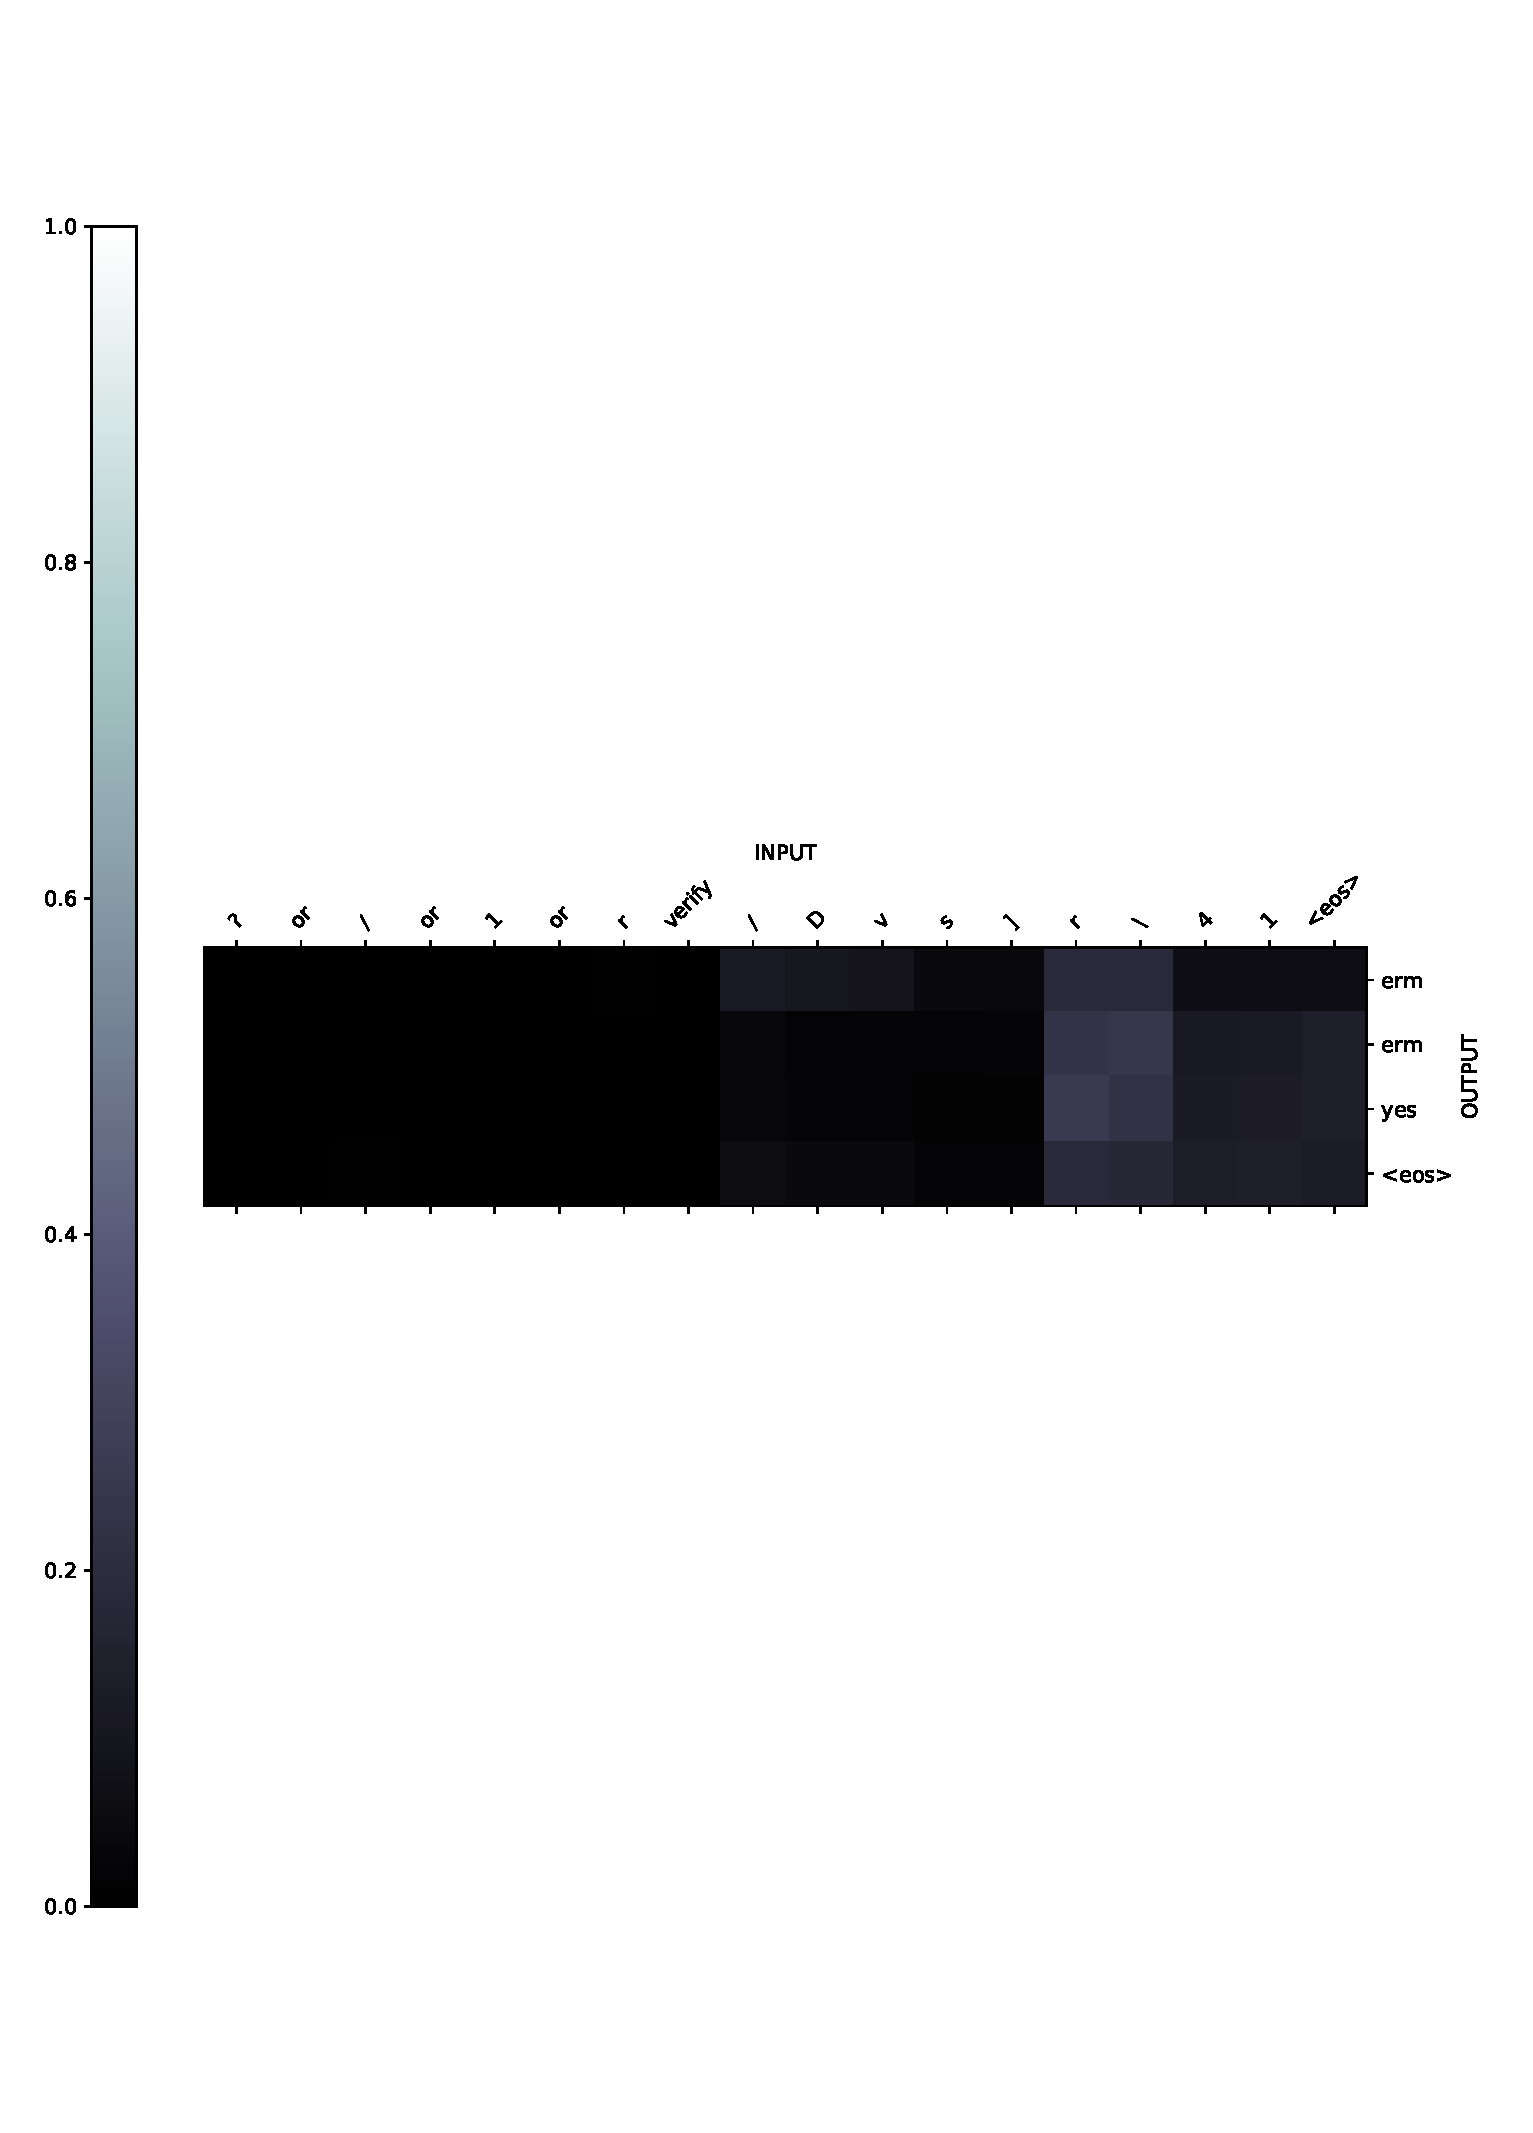
\includegraphics[width=0.95\linewidth]{./figs/micro/base-verify-eps}
		\caption{Verify} 
		\label{base-ver} 
		\vspace{2ex}
	\end{subfigure}%% 
	\begin{subfigure}[b]{0.5\linewidth}
		\centering
		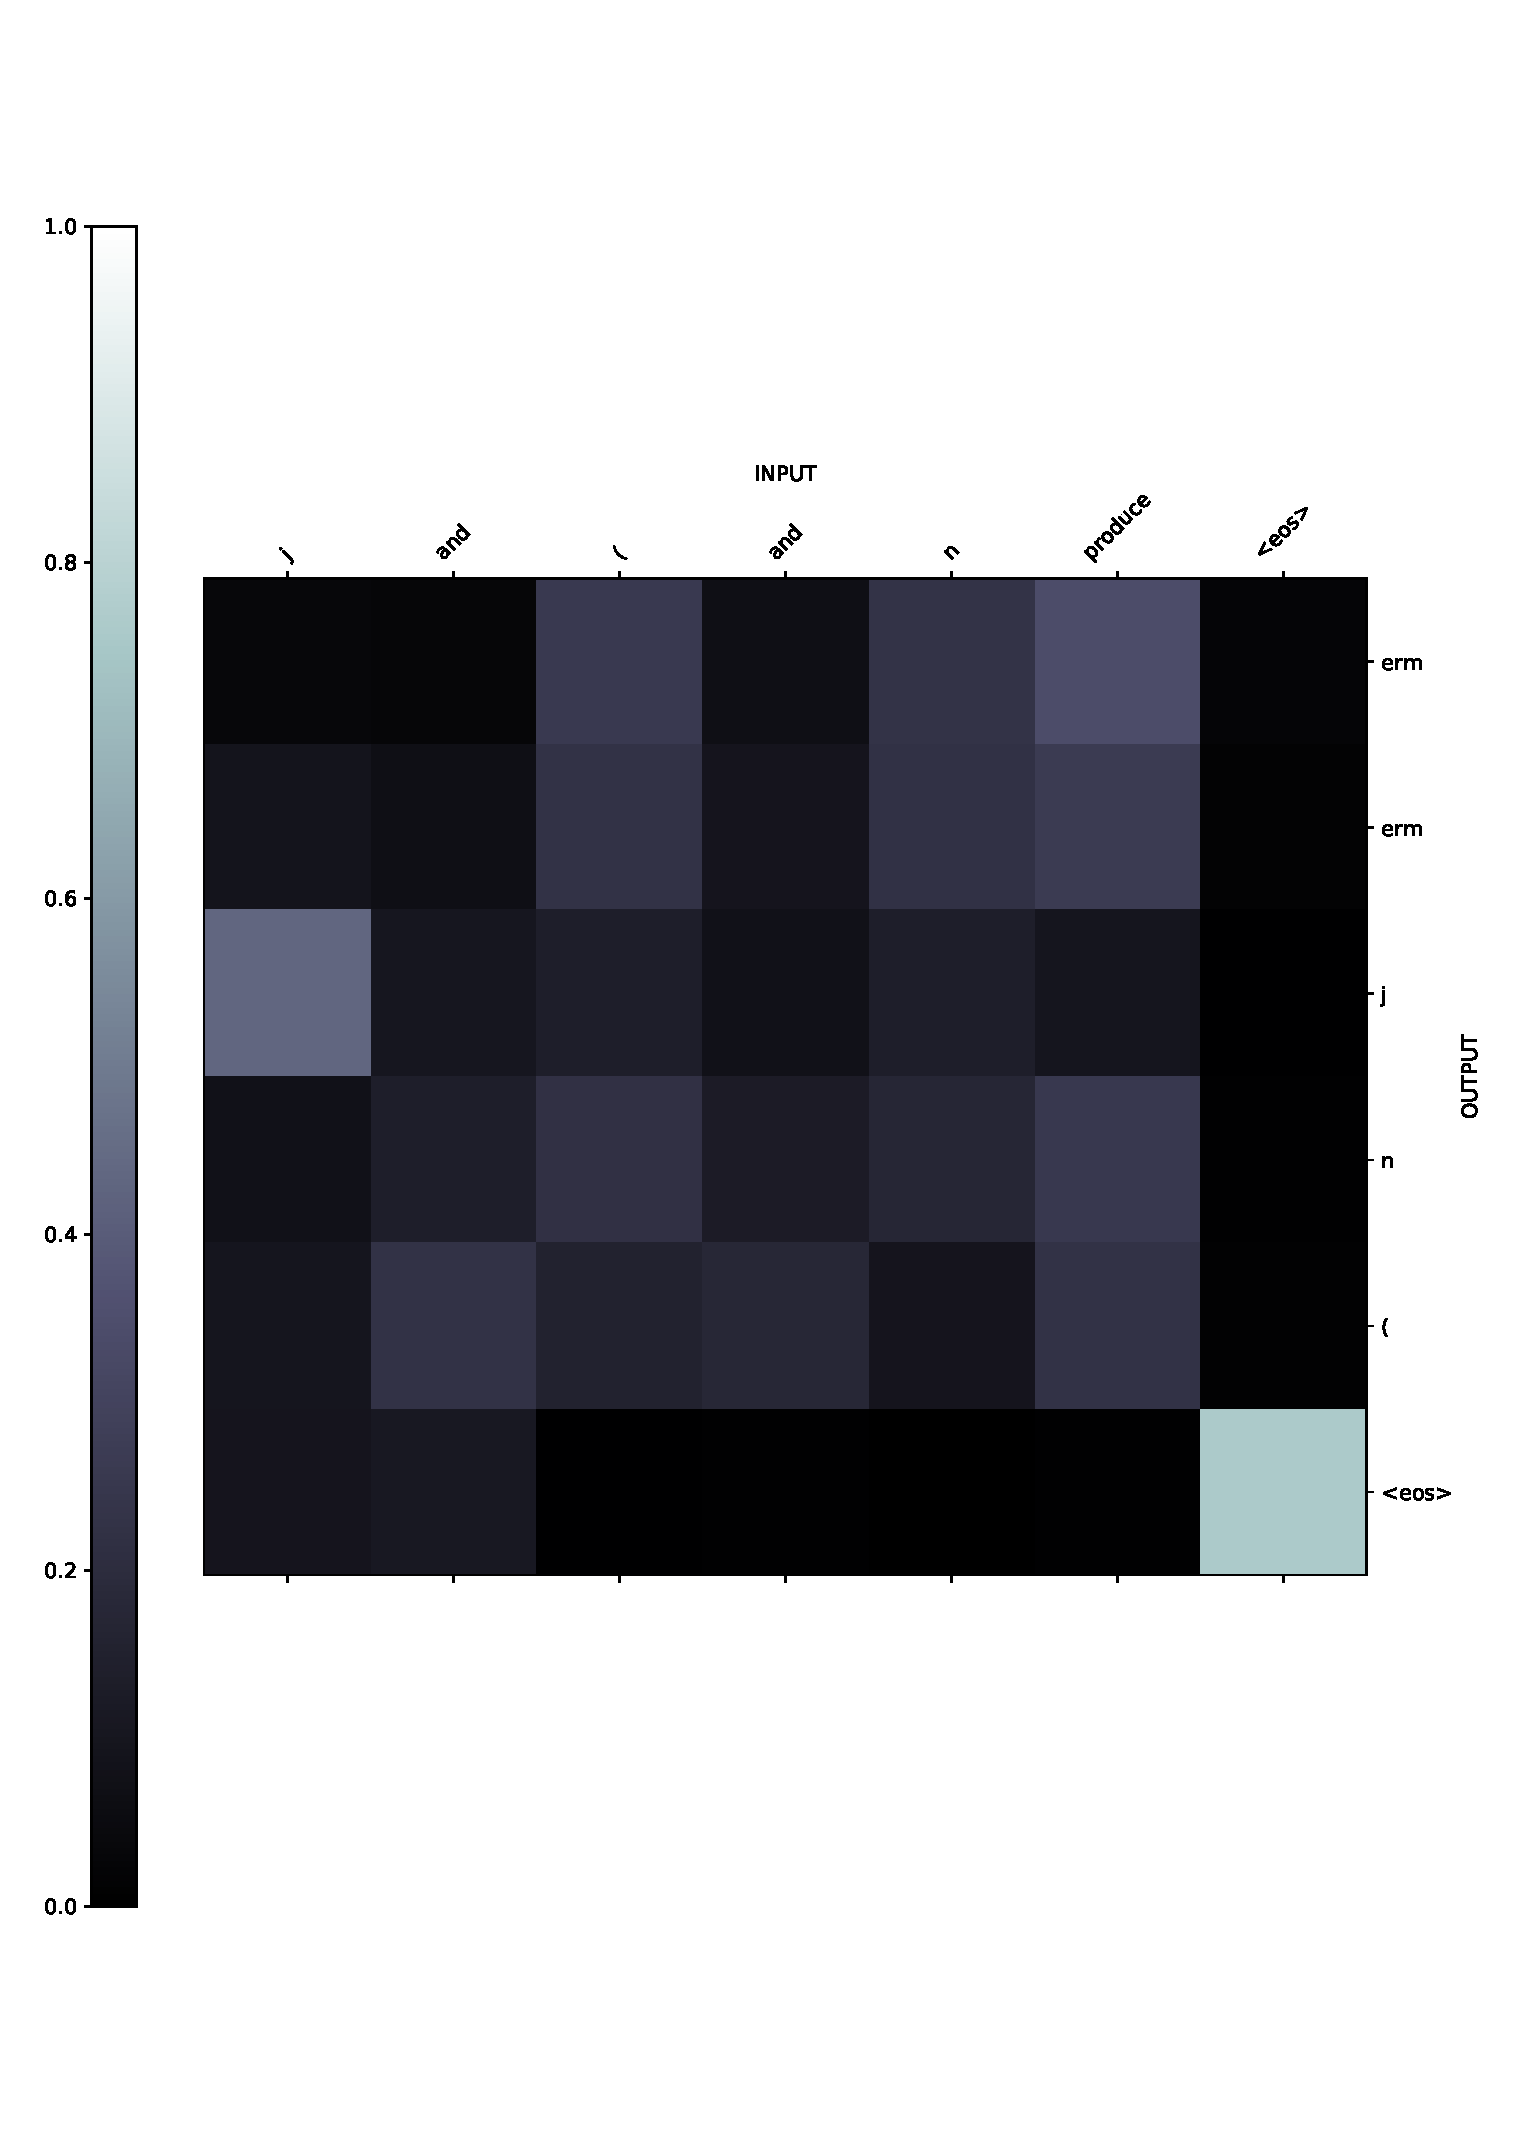
\includegraphics[width=0.95\linewidth]{./figs/micro/base-prod-eps}
		\caption{Produce} 
		\label{base-prod} 
		\vspace{2ex}
	\end{subfigure}
	\caption{Attention plots for baseline on both verify and produce tasks. }
	\label{base-attn}
\end{figure}
The baseline clearly fails on the production tasks, as does the learned guidance. Unsurprisingly \lq or\rq{} is the easiest operation production task even for longer and unseen-longer test splits. (figures \ref{mtu2}, \ref{mtl2} and \ref{mtul2}). A probable explanation for this the fact that a model can solve an \lq or\rq{} task just by emitting a subsection of the longer string and thus increasing the length is inconsequential. The reason(s) behind the models performing better on \lq and\rq{} as compared to \lq not\rq{} is not clear and is left as future work.

\begin{figure}[H] 
	\begin{subfigure}[b]{0.5\linewidth}
		\centering
		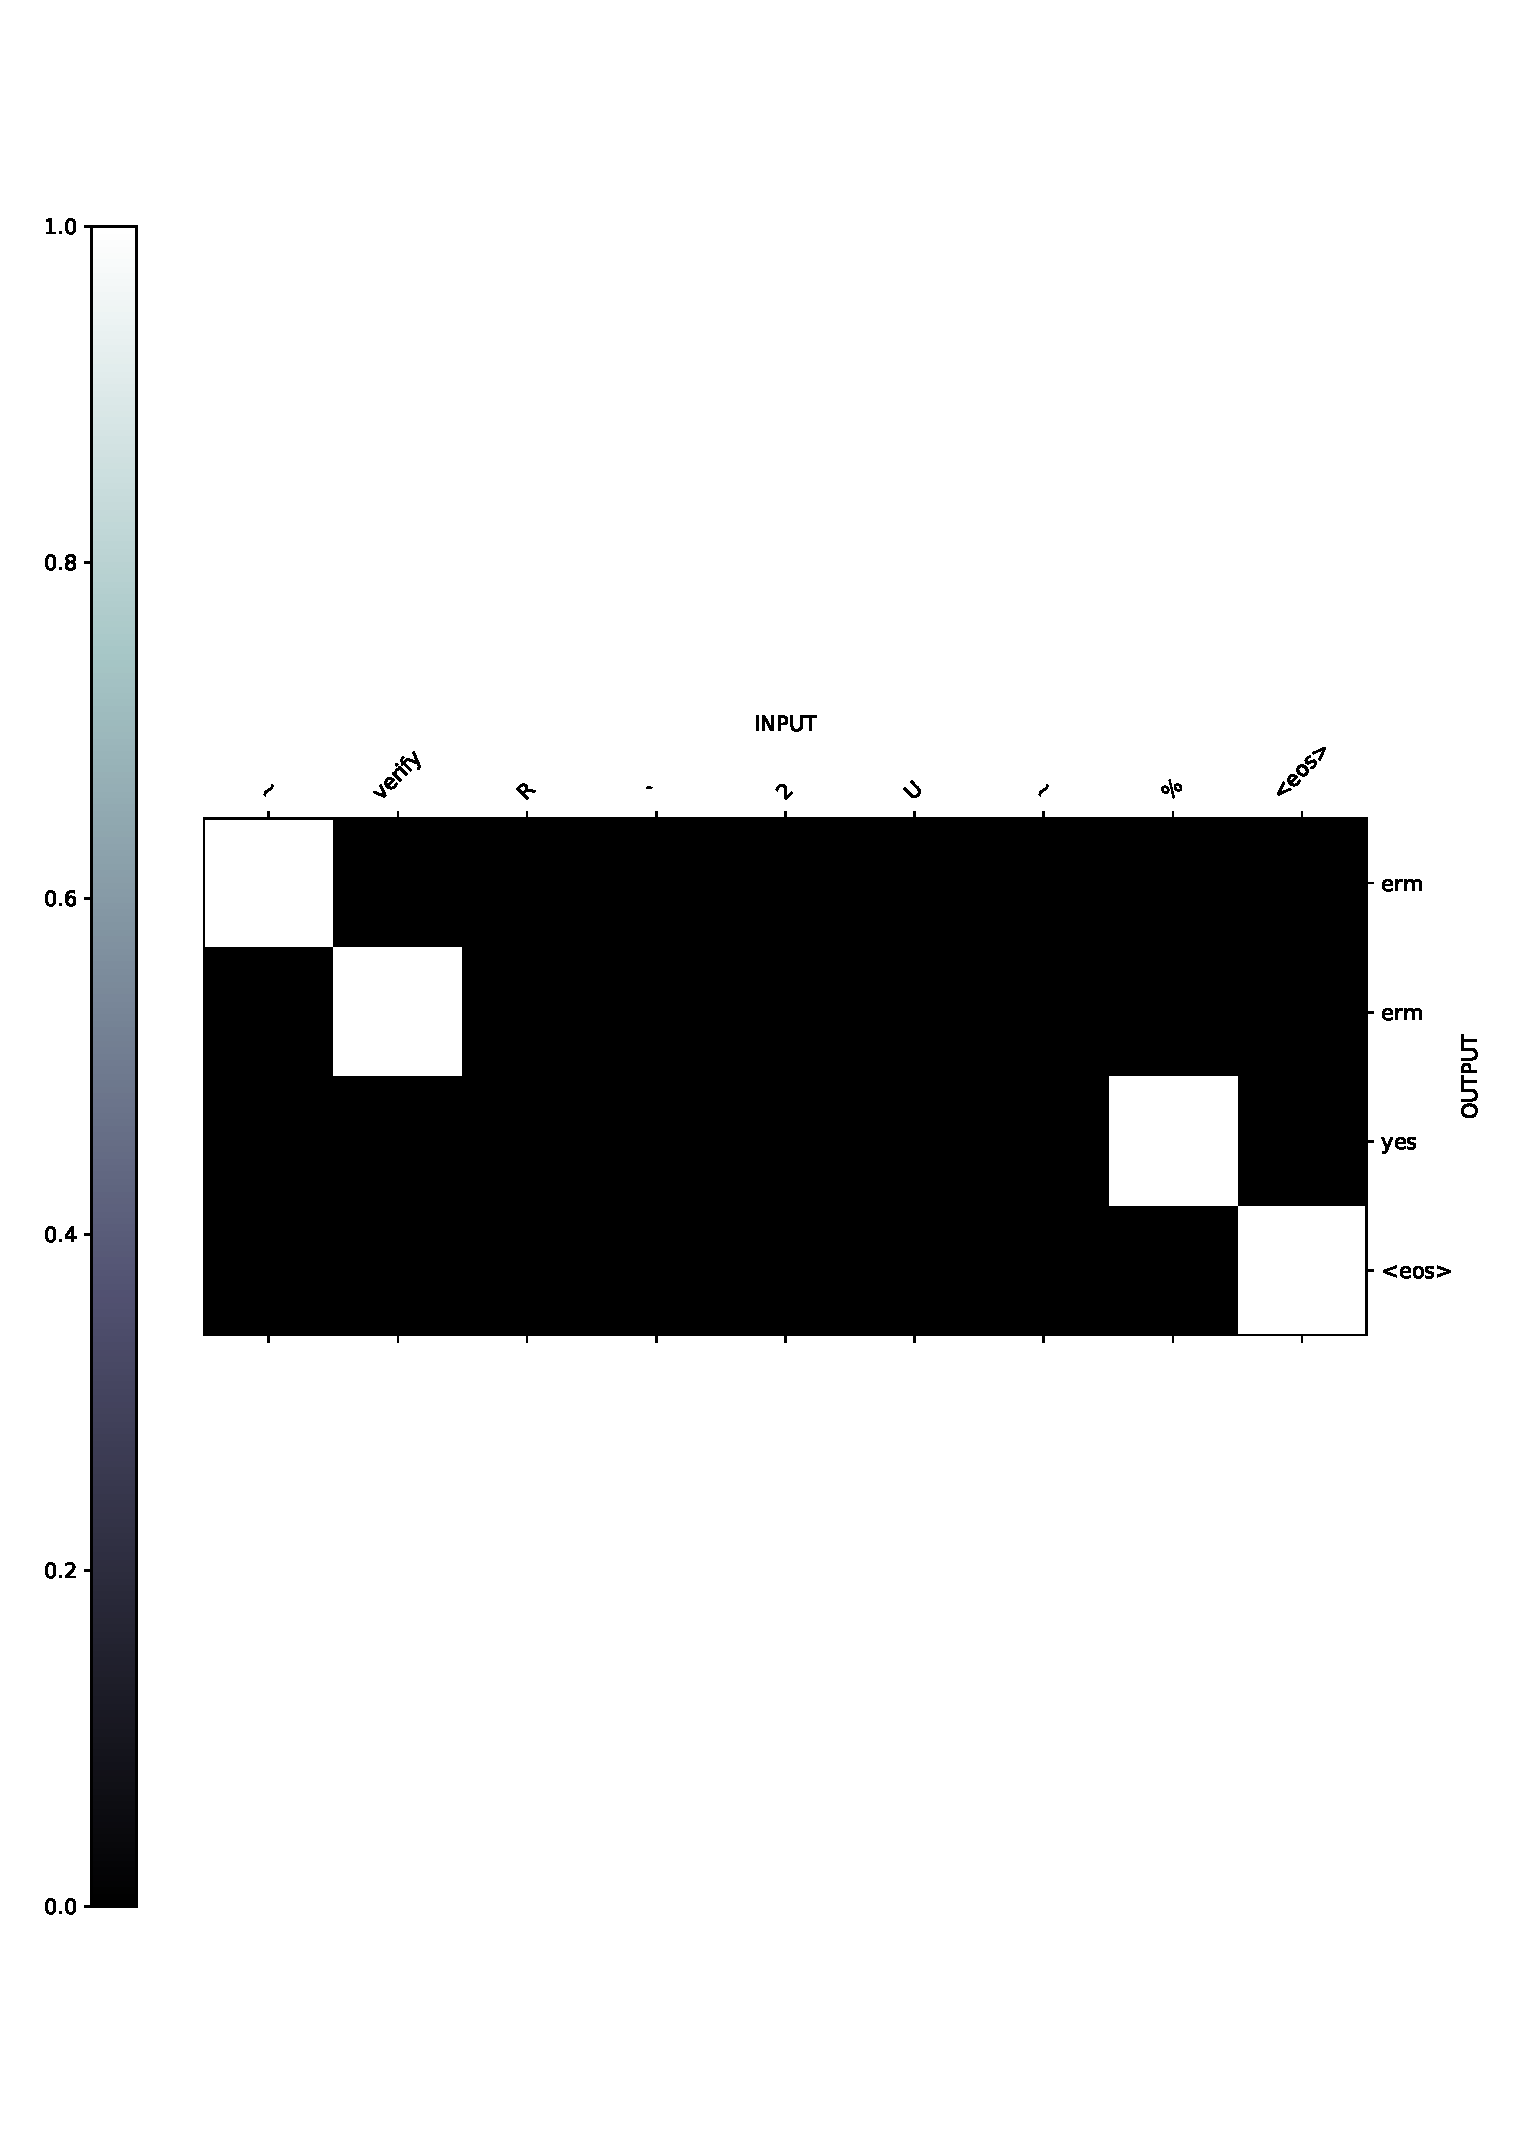
\includegraphics[width=0.95\linewidth]{./figs/micro/learn-ver-eps}
		\caption{Verify} 
		\label{learn-ver} 
		\vspace{2ex}
	\end{subfigure}%% 
	\begin{subfigure}[b]{0.5\linewidth}
		\centering
		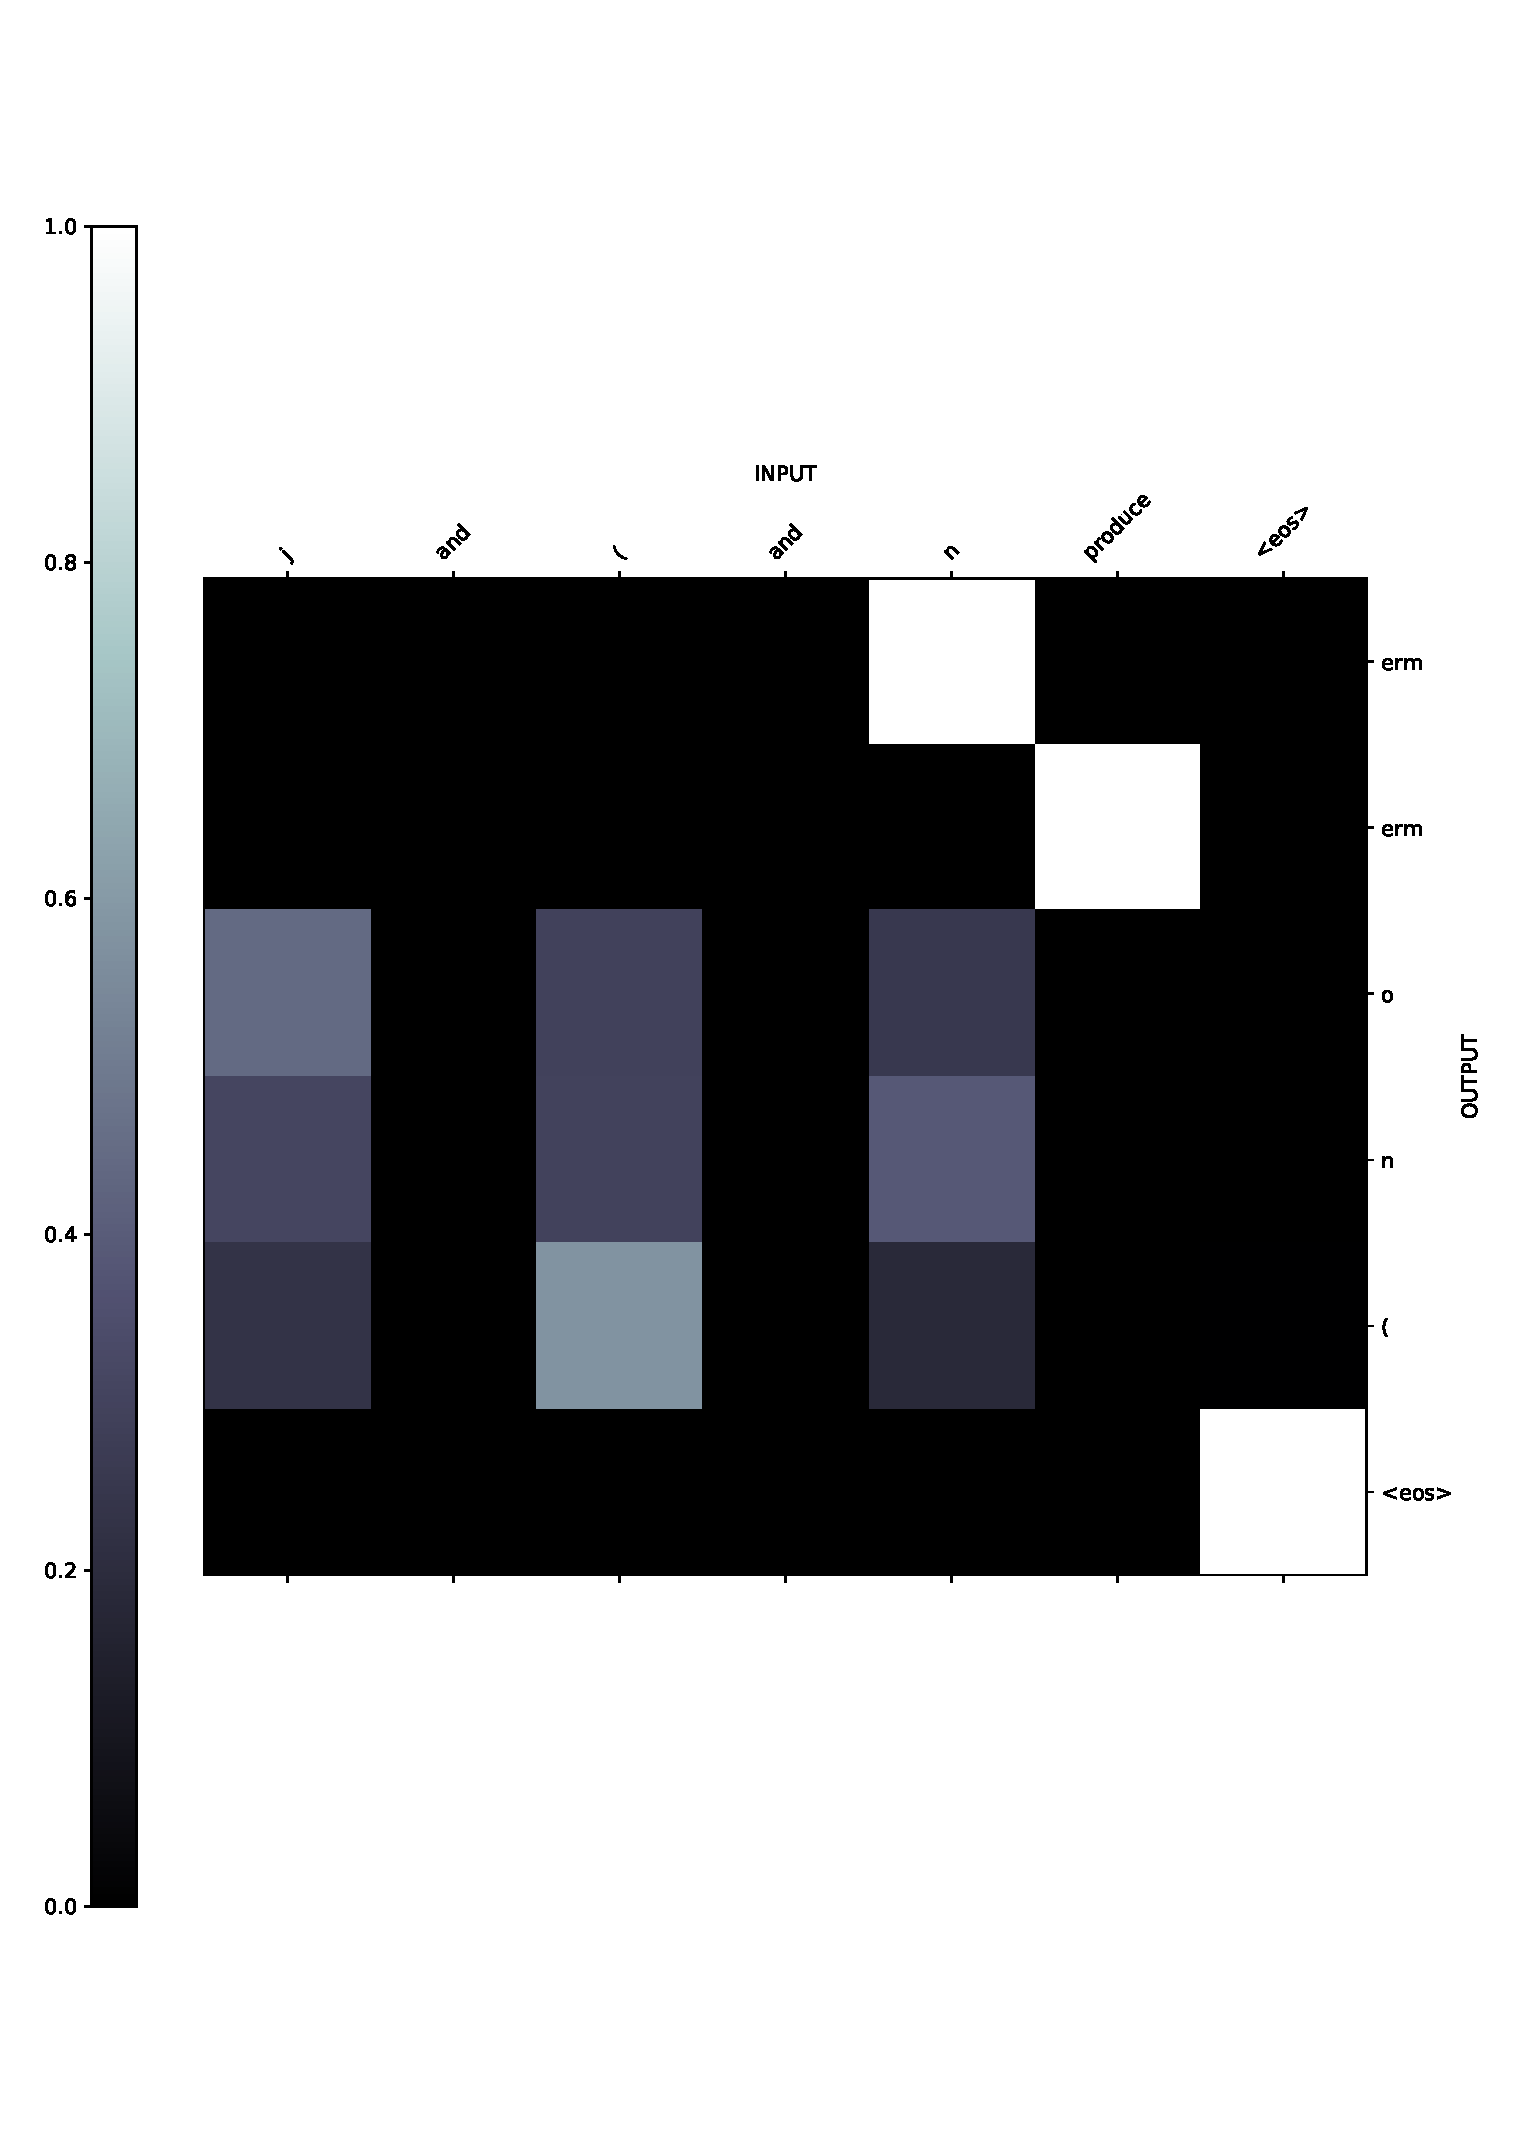
\includegraphics[width=0.95\linewidth]{./figs/micro/learn-prod-eps}
		\caption{Produce} 
		\label{learn-prod} 
		\vspace{2ex}
	\end{subfigure}
	\caption{Attention plots for AG model on both verify and produce tasks. }
	\label{learn-attn}
\end{figure}

\section{Discussion}\label{mt:disc}
The huge chasm between the performance of the models with attentive guidance and hard guided models again brings to fore the argument I raised in section \ref{pm:disc}, that the current architectural setting is not optimal for learning the correct trace. This is substantiated by the attention plot for learned model in figure \ref{learn-prod}. The model's attention is diffused over the three target emissions and it leads to one wrong emission in the sequence. One striking observation from the attention plot of baseline for verification task (figure \ref{base-ver}) is that it utilizes only the witness string to make its decision.

It has already been discussed in the introduction to this chapter that the language $L$ proposed in this dataset $\notin NP$. However even for this language the results indicate that search (production) is more difficult than decision (verification) for a prover (a vanilla seq2seq model in our case). But the same vanilla seq2seq with additional hardcoded attention vectors can solve the search problem to a reasonable degree. This warrants additional investigation for effectiveness of hard guidance in languages which are higher up in the polynomial hierarchy \citep{arora2009computational}.  